\documentclass[12pt]{article}
\usepackage[utf8]{vietnam}
\usepackage{amsmath}
\usepackage{amsfonts}
\usepackage{amssymb}
\usepackage{amsopn}
\usepackage{amsthm}
\usepackage{commath}
\usepackage{graphicx}
\usepackage{subcaption}
\usepackage{amsxtra}
\usepackage{indentfirst}
\usepackage{pdfpages}
\usepackage[sort&compress]{natbib}
\usepackage{wasysym}
\usepackage{mathtools}
\usepackage{physics}
\usepackage[mathscr]{eucal}

\DeclareMathOperator{\spn}{span}
\DeclareMathOperator{\dis}{d}
% \DeclareMathOperator{\rank}{rank}
\newcommand{\R}{\mathbb{R}}
\newcommand{\N}{\mathbb{N}}
\newcommand{\K}{\mathbb{K}}
\newcommand{\C}{\mathbb{C}}
\newcommand{\codim}{\operatorname{codim}}
\newcommand{\olsi}[1]{\,\overline{\!{#1}}}
\newtheorem{lemma*}{Bổ đề}
\newtheorem{theorem}{Định lý}
\newtheorem{proposition}{Bài}
\newtheorem{corollary*}{Chứng minh}
\newenvironment{solution}{%
     \setlength\parindent{0pt}\par\medskip\textbf{Lời giải.}\quad}{%
     \hfill\tiny$\blacksquare$\par\medskip}
\usepackage[left=2cm,right=2cm,top=2cm,bottom=2cm]{geometry}
\setlength{\parindent}{0pt}

\begin{document}
    Thông tin các thành viên trong nhóm 5:
    \begin{enumerate}
        \item[1.] Lê Thị Thu An, 18001975, K63 TN Toán học.
        \item[2.] Thiều Đình Minh Hùng, 21000006, K66 TN Toán học.
    \end{enumerate}
    \begin{center}
        $*********$
    \end{center}
    \textbf{Bài tập 1.} Những hàm sau đây là hàm lồi hay không? Đưa ra chứng minh hoặc phản ví dụ.
    \begin{enumerate}
        \item[1.] $f(x) = a^x$ với $x \in \R$ và tham số $a > 0$.
        \item[2.] $g(x) = a^{T}x + b$ với $x \in \R^n$ và tham số $a, b \in \R^n$.
        \item[3.] $h(x) = \norm{y - Ax}_2^2$ với $x \in \R^n$ và tham số $y \in \R^m, A \in \R^{m \times n}$.
        \item[4.] $k(x) = \max\{x_1, x_2, \dots, x_n\}$ với $x = (x_1 \quad x_2 \quad \ldots \quad x_n)^T \in \R^n$.
        \item[5.] $l(x) = \min\{x_1, x_2, \dots, x_n\}$ với $x = (x_1 \quad x_2 \quad \ldots \quad x_n)^T \in \R^n$.
    \end{enumerate}
    \begin{solution}
        \begin{enumerate}
            \item[1.] Xét hai trường hợp:
            \\
            - Nếu $a = 1$ thì $f \equiv 1$. Dễ thấy hàm này là hàm lồi.
            \\
            - Nếu $a \neq 1$ thì $f$ khả vi vô hạn lần và:
            \begin{align*}
                f'(x) = \ln a \cdot a^x \Rightarrow f''(x) = (\ln a)^2 \cdot a^x > 0 \quad \forall x \in \R.
            \end{align*}
            Do đó, $f$ là hàm lồi.
            \item[2.] Để ý rằng:
            \begin{align*}
                g(\lambda x_1 + (1 - \lambda)x_2) &= a^T(\lambda x_1 + (1 - \lambda)x_2) + b\\
                &= \lambda(a^Tx_1 + b) + (1 - \lambda)(a^Tx_2 + b)\\
                &= \lambda g(x_1) + (1 - \lambda)g(x_2), \quad \forall x_1, x_2 \in \R^n, \lambda \in [0, 1].
            \end{align*}
            Suy ra $g$ là hàm lồi.
            \item[3.] Theo BĐT Cauchy - Schwarz ta có:
            \begin{align*}
                \lambda h(x_1) + (1 - \lambda)h(x_2) &= \bigl(\lambda h(x_1) + (1 - \lambda)h(x_2)\bigr) (\lambda + (1 - \lambda))\\
                &\geq (\lambda h(x_1) + (1 - \lambda)h(x_2))^2\\
                &= (\norm{\lambda y - \lambda Ax_1}_2 + \norm{(1 - \lambda)y - (1 - \lambda)Ax_2}_2)^2\\
                &\geq (\norm{\lambda y - \lambda Ax_1 + (1 - \lambda)y - (1 - \lambda)Ax_2}_2)^2\\
                &= h(\lambda x_1 + (1 - \lambda)x_2), \quad \forall x_1, x_2 \in \R^n, \lambda \in [0, 1].
            \end{align*}
            Suy ra $h$ là hàm lồi.
            \item[4.] Xét $x^{(0)} = (x_1^{(0)} \quad x_2^{(0)} \quad \ldots \quad x_n^{(0)})^T, y^{(0)} = (y_1^{(0)} \quad y_2^{(0)} \quad \ldots \quad y_n^{(0)})^T \in \R^n$ và $\lambda \in [0, 1]$ tùy ý.
            \\
            Đặt $z^{(0)} = \lambda x^{(0)} + (1 - \lambda)y^{(0)} = (z_1^{(0)} \quad z_2^{(0)} \quad \ldots \quad z_n^{(0)})^T$ và giả sử rằng $z_{i_0}^{(0)} = k(z^{(0)})$. Khi đó:
            \begin{align*}
                k(\lambda x^{(0)} + (1 - \lambda)y^{(0)}) = k(z^{(0)}) = z_{i_0}^{(0)} = \lambda x_{i_0}^{(0)} + (1 - \lambda)y_{i_0}^{(0)} \leq \lambda k(x^{(0)}) + (1 - \lambda)k(y^{(0)}).
            \end{align*}
            Suy ra $k$ là hàm lồi.
            \item[5.] Hàm này không phải hàm lồi, vì với $x^{(0)} = (1 \quad 0 \quad \ldots \quad 0)^T, y^{(0)} = (0 \quad 1 \quad \ldots \quad 1)^T \in \R^n$ và $\lambda = \frac{1}{2}$, ta có:
            \begin{align*}
                l(\lambda x^{(0)} + (1 - \lambda)y^{(0)}) = l \Bigl(\bigl(\frac{1}{2} \quad \frac{1}{2} \quad \ldots \quad \frac{1}{2}\bigr)^T\Bigr) = \frac{1}{2} > 0 = \frac{1}{2}(l(x^{(0)}) + l(y^{(0)})).
            \end{align*}
        \end{enumerate}
    \end{solution}
    \textbf{Bài tập 2.} Cho hàm số $f(x, y) = x^4 - x^2 + 14xy + y^2$. Hãy tìm các điểm cực trị địa phương của $f$, hãy chỉ rõ đó là cực đại hay cực tiểu địa phương.
    \begin{solution}
        \\
        Để ý rằng $f \in C^{\infty}(\R^2, \R)$. Ta có:
        \begin{align*}
            \begin{cases}
                \frac{\partial f}{\partial x} = 4x^3 - 2x + 14y, \quad \frac{\partial f}{\partial y} = 14x + 2y\\
                \frac{\partial^2 f}{\partial x^2} = 12x^2 - 2, \quad \frac{\partial^2 f}{\partial y^2} = 2, \quad \frac{\partial^2 f}{\partial x \partial y} = \frac{\partial^2 f}{\partial y \partial x} = 14.
            \end{cases}
        \end{align*}
        Như vậy:
        \begin{align*}
            \nabla f(x, y) = \begin{pmatrix}
                0\\
                0
            \end{pmatrix} &\Leftrightarrow \begin{cases}
                4x^3 - 2x + 14y = 0\\
                14x + 2y = 0
            \end{cases}\\
            &\Leftrightarrow \begin{cases}
                4x^3 - 100x = 0\\
                y = -7x
            \end{cases}\\
            & \Leftrightarrow (x,y) \in {(0, 0), (5, -35), (-5, 35)}.
        \end{align*}
        Ma trận Hessian của $f$ tại $(x, y)$ là:
        \begin{align*}
            H_f(x, y) = \begin{pmatrix}
                12x^2 - 2 & 14\\
                14 & 2
            \end{pmatrix}.
        \end{align*}
        - Với $(x, y) = (0, 0)$, ta có $H_f(0, 0) = \begin{pmatrix}
            -2 & 14\\
            14 & 2
        \end{pmatrix}$.
        \\
        Để ý rằng $\det{H_f(0, 0)} = -200 < 0$. Do đó, ma trận $H_f(0, 0)$ không xác định dấu, tức là $(0, 0)$ không phải là điểm cực trị của $f$.
        \\
        - Với $(x, y) = (5, -35)$, ta có $H_f(5, -35) = \begin{pmatrix}
            298 & 14\\
            14 & 2
        \end{pmatrix}$.
        \\
        Để ý rằng $\det{H_f(5, -35)} = 2 \cdot 298 - 14^2 > 0$ và $\frac{\partial^2 f}{\partial x^2}(5, -35) = 298 > 0$. Do đó, ma trận $H_f(5, -35)$ xác định dương, tức là $(5, -35)$ là điểm cực tiểu địa phương của $f$.
        \\
        - Với $(x, y) = (-5, 35)$, ta có $H_f(-5, 35) = \begin{pmatrix}
            298 & 14\\
            14 & 2
        \end{pmatrix}$.
        \\
        Để ý rằng $\det{H_f(-5, 35)} = 2 \cdot 298 - 14^2 > 0$ và $\frac{\partial^2 f}{\partial x^2}(-5, 35) = 298 > 0$. Do đó, ma trận $H_f(-5, 35)$ xác định dương, tức là $(-5, 35)$ là điểm cực tiểu địa phương của $f$.
        \\
        Như vậy, $f$ có hai điểm cực trị địa phương là $(5, -35)$ và $(-5, 35)$, các điểm này đều là điểm cực tiểu địa phương của $f$.
    \end{solution}
    \textbf{Bài tập 3.} Cho $A \in \R^{m \times n}$ với $m > n$ và $\rank{(A)} = n$. Hãy giải bài toán tối ưu sau:
    \begin{align*}
        \min\limits_{x} {\norm{Ax - b}_2^2}.
    \end{align*}
    \\
    \textbf{Bài tập 4.} Trong bài tập này, ta nghiên cứu cách mô hình hóa điều kiện phi tuyến, cụ thể là
    phép nhân, bởi các ràng buộc tuyến tính.
    \begin{enumerate}
        \item[1.] Cho $A \in \R^{m \times n}, b \in \R^m$. Chứng minh tập hợp $S = \{x \in \R^n \mid Ax \leq b\}$ là một tập lồi.
        \item[2.] Cho $A \in \R^{m \times n}, b \in \R^m$. Chứng minh tập hợp $S = \{x \in \R^n \mid Ax = b\}$ là một tập lồi.
        \item[3.] Cho ba biến nhị phân $x, y, z$ thỏa mãn $x.y = z$. Liệt kê tất cả các giá trị có thể của bộ ba $(x, y, z)$.
        \item[4.] Cho ba biến nhị phân $x, y, z$. Mô tả điều kiện $x.y = z$ bởi các ràng buộc tuyến tính giữa ba biến $x, y, z$.
        \item[5.] Cho một số nguyên dương $m$ và ba biến nguyên $x, y, z$ thỏa mãn $x$ là một biến nhị phân và $y, z \in \{0, 1, \dots, m\}$. Mô tả điều kiện $x.y = z$ bởi các ràng buộc tuyến tính giữa ba biến $x, y, z$.
        \item[6.] Cho ba biến nguyên $x, y, z$ thỏa mãn $x, y \in \{0, 1, 2\}$ và $z \in \{0, 1, 2, 3, 4\}$. Chứng minh không thể mô tả điều kiện $x.y = z$ chỉ bằng các ràng buộc tuyến tính giữa ba biến $x, y, z$.
        \item[7.] Cho ba biến nguyên $x, y, z$ thỏa mãn $x, y \in \{0, 1, 2\}$ và $z \in \{0, 1, 2, 3, 4\}$. Hãy mô tả điều kiện $x.y = z$ chỉ bằng các ràng buộc tuyến tính.
    \end{enumerate}
    %chèn thêm bai3_va_bai4.pdf
    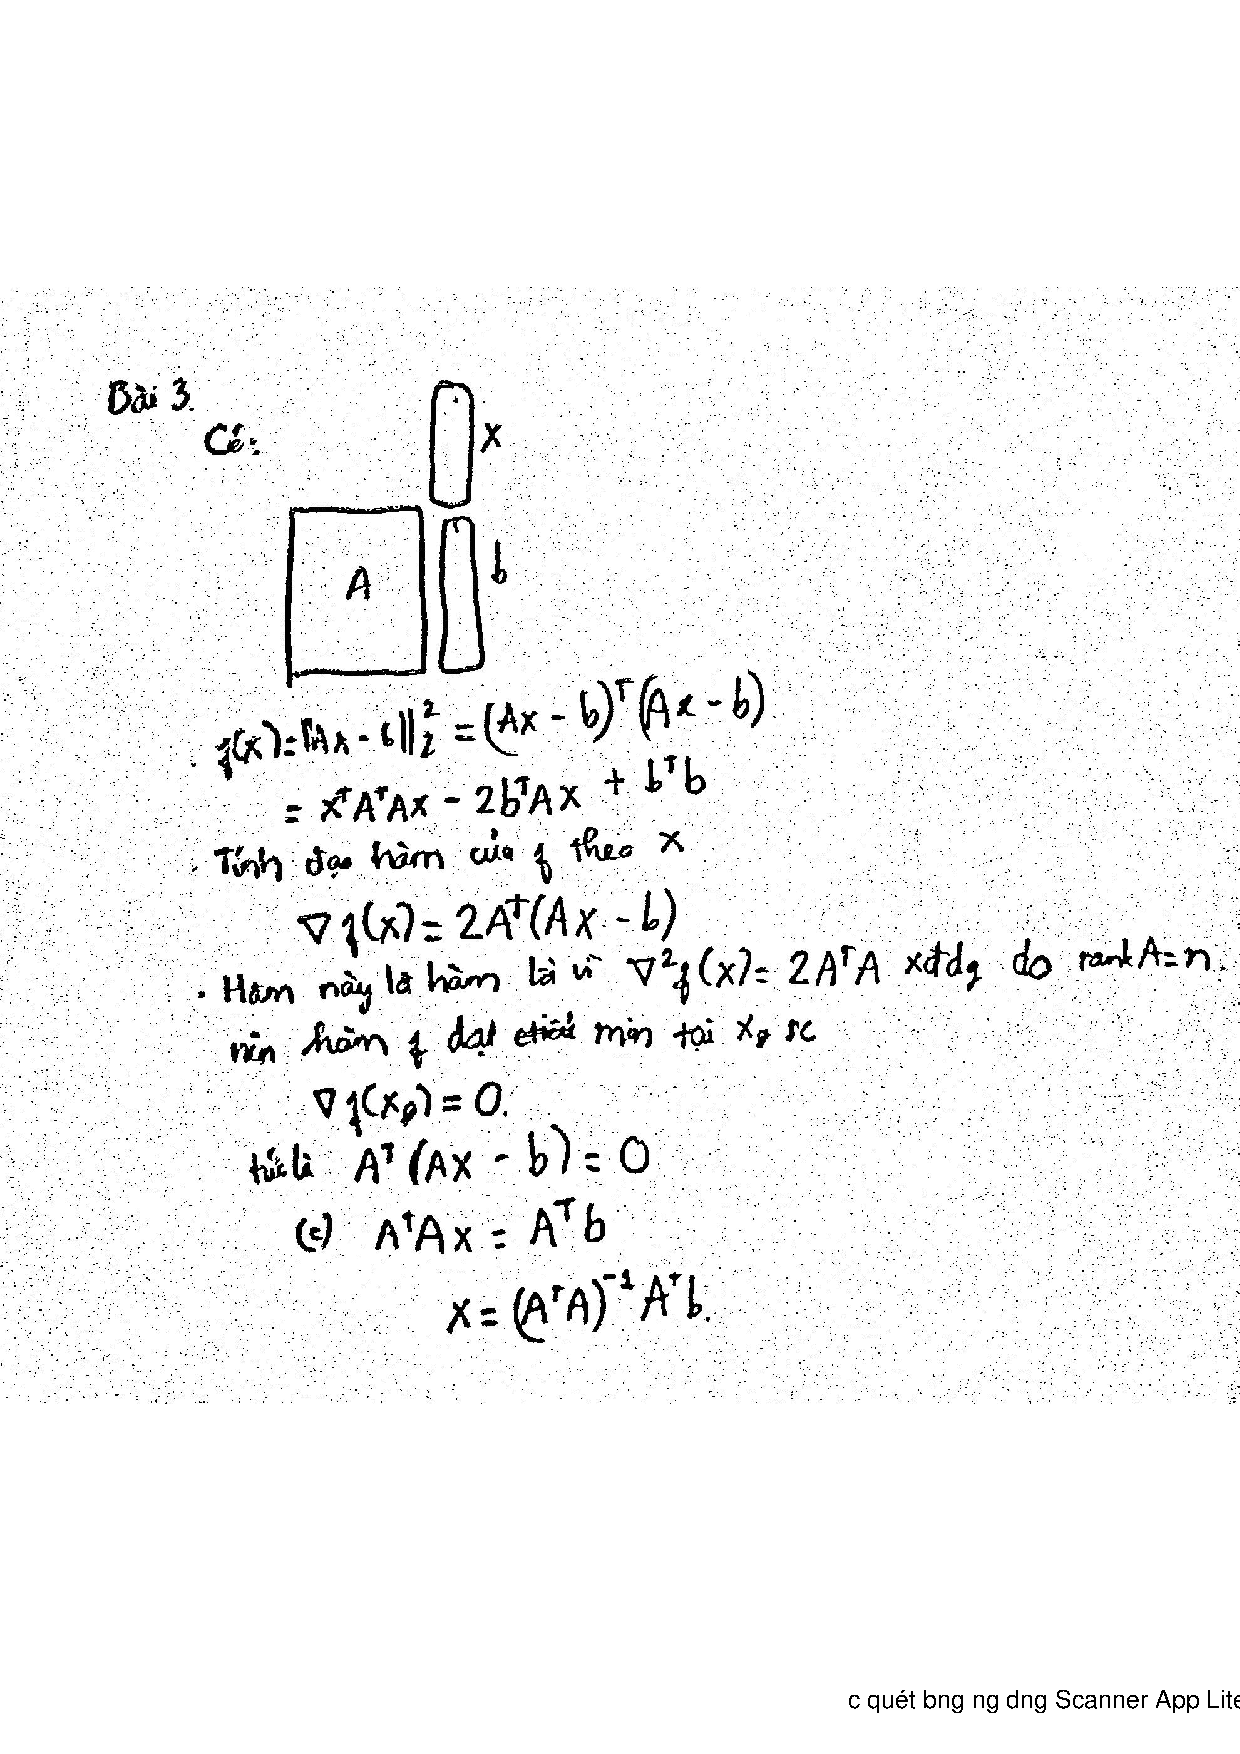
\includepdf[pages=-]{bai3_va_4.pdf}

    \textbf{Bài tập 5.} (Circle packing in a square)
    \\
    Cho N là một số nguyên dương. Biết rằng có thể đặt N hình tròn đơn vị vào trong một
    hình vuông cạnh d sao cho hai hình tròn bất kỳ không có phần trong chung. Tìm giá trị nhỏ nhất
    của d.

    Xây dựng mô hình tối ưu phi tuyến giải quyết bài toán trên.
    

\end{document}
